%! Author = Adrian Helberg

% Preamble
\documentclass[12pt]{beamer}
% Theme
\usetheme{Boadilla}

% Bibliography
\bibliography{literature}
\bibliographystyle{plain}

% Packages
\usepackage{amsmath}
\usepackage[utf8]{inputenc}
\usepackage{ngerman}
\usepackage{graphicx}
\usepackage{color}
\usepackage{xcolor}
\usepackage[export]{adjustbox}
\usepackage{algorithm2e}
\usepackage{algpseudocode}

% Remove frame break numbering
\setbeamertemplate{frametitle continuation}{}

\subtitle{Template-basierte Synthese von\\Verzweigungsstrukturen mittels L-Systemen}
\title{Bachelorarbeit Kolloquium}
\author{Adrian Helberg}
\institute{HAW Hamburg}
\date{\today}
\titlegraphic{
\includegraphics[scale=0.25]{../images/HAW_Marke_CMYK.pdf}}

% Document
\begin{document}
    \frame{\titlepage}
    \frame{\frametitle{Agenda} \tableofcontents}

    \section{Einleitung}
    \label{sec:thema}
    \begin{frame}[allowframebreaks]
        \frametitle{Einleitung: Titel}

        \begin{block}{Titel}
            \color{olive}\underline{\color{black}Template-basierte} \color{teal}\underline{\color{black}Synthese} 
            \color{black}von \color{orange}\underline{\color{black}Verzweigungsstrukturen} \color{black}mittels 
            \color{cyan}\underline{\color{black}L-Systemen}
        \end{block}

        \begin{itemize}
            \item[\color{olive}$\rightarrow$] \color{black}Verschiedene Muster als kleinste zu organisierende Einheit
            \item[\color{teal}$\rightarrow$] \color{black}Verknüpfung von Verzweigungen zu einer neuen Struktur
            \item[\color{orange}$\rightarrow$] \color{black}Baumstrukturen als Ergebnis der Synthese
            \item[\color{cyan}$\rightarrow$] \color{black}Formale Grammatik zur Kodifizierung von Strukturen
        \end{itemize}
    \end{frame}

    \begin{frame}
        \frametitle{Einleitung: Relevanz}

        \begin{figure}
            \centering
            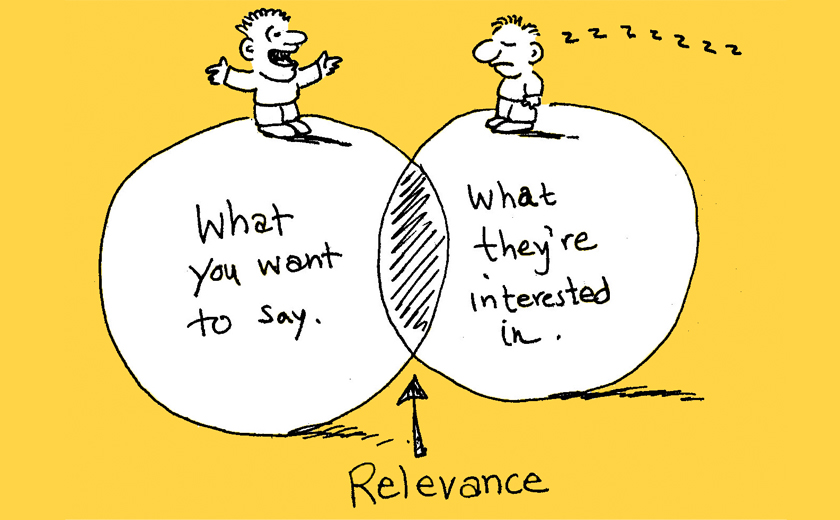
\includegraphics[width=10cm]{../images/relevanz.jpg}
        \end{figure}
    \end{frame}

    \begin{frame}
        \frametitle{Einleitung: Relevanz}

        \begin{itemize}
            \setlength\itemsep{1em}
            \item<1-> Digitalisierung
            \item<2-> Kein einsteigerfreundliches Gebiet
            \item<3-> Automatisierte Erstellung von digitalen Inhalten
            \begin{itemize}
                \item "`Natürlichkeit der Dinge"'
            \end{itemize}
            \item<4-> Regeln und Muster kodifizieren
            \item<5-> Künstliche Intelligenz
        \end{itemize}
    \end{frame}

    \begin{frame}
        \frametitle{Einleitung: Ziele}

        \begin{figure}
            \centering
            
\includegraphics[width=10cm]{../images/ziel.jpeg}
        \end{figure}
    \end{frame}

    \begin{frame}
        \frametitle{Einleitung: Ziele}

        \begin{block}{Zentrale Aufgabe}
            System zur Umsetzung einer Synthese von Strukturen, die einer Eingabestruktur ähneln
        \end{block}

        \begin{itemize}
            \setlength\itemsep{1.4em}
            \item<2-> Methodiken und Algorithmen aus der aktuellen Forschung
            \begin{itemize}
                \item Praktikabilität
                \item Anwendung am Beispiel eines Programms
            \end{itemize}
            \item<3-> Erzeugen von Ähnlichkeit
            \item<4-> Automatisierte Erstellung
        \end{itemize}
    \end{frame}

    \section{Forschung}
    \label{sec:forschung}
    \begin{frame}
        \frametitle{Forschung: Verwandte Arbeiten}

        \begin{figure}
            \centering
            
\includegraphics[width=10cm]{../images/forschung.jpg}
        \end{figure}
    \end{frame}

    \begin{frame}
        \frametitle{Forschung: Verwandte Arbeiten}

        \begin{figure}
            \centering
            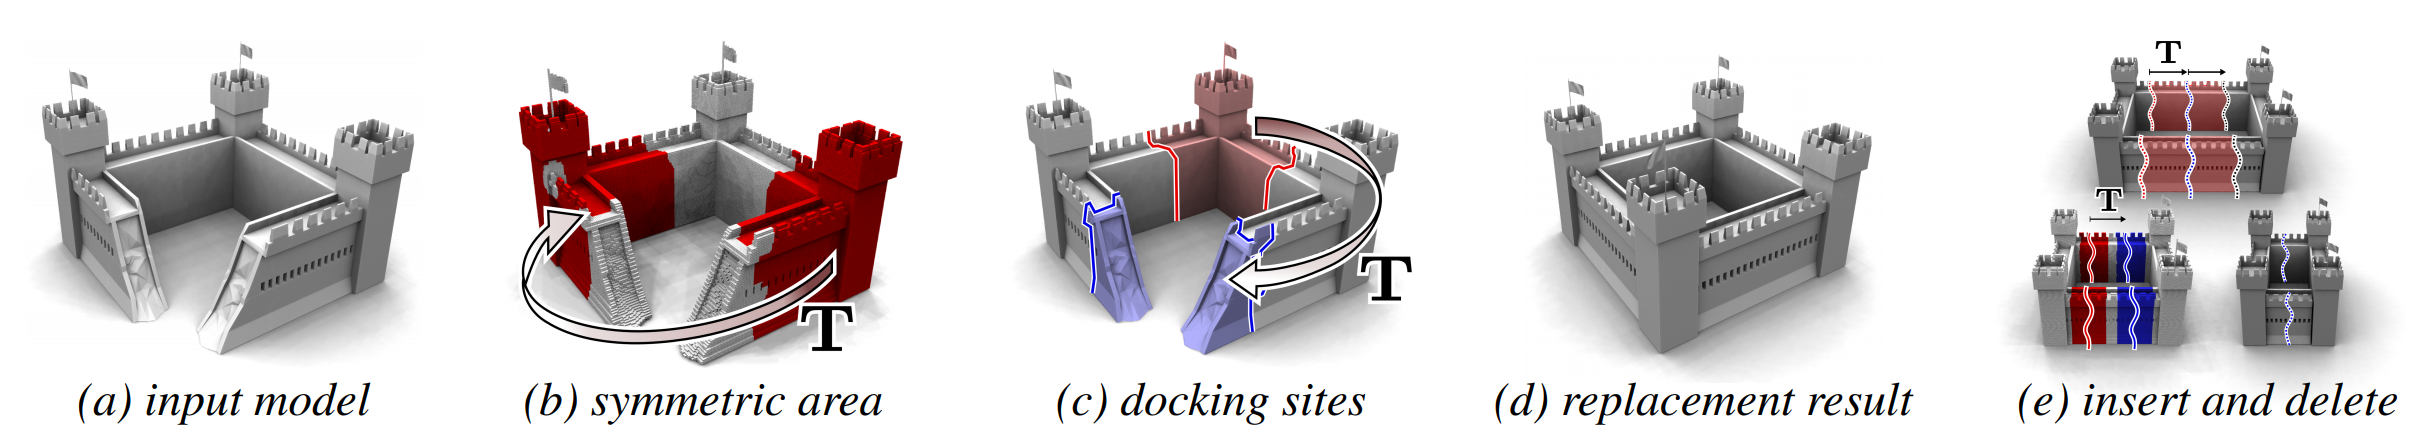
\includegraphics[width=12cm]{../images/bokeloh_2010_system.PNG}
            \caption{Textur- und Geometriesynthese anhand lokaler Ähnlichkeit}
        \end{figure}
    \end{frame}

    \begin{frame}
        \frametitle{Forschung: Verwandte Arbeiten}

        \begin{figure}
            \centering
            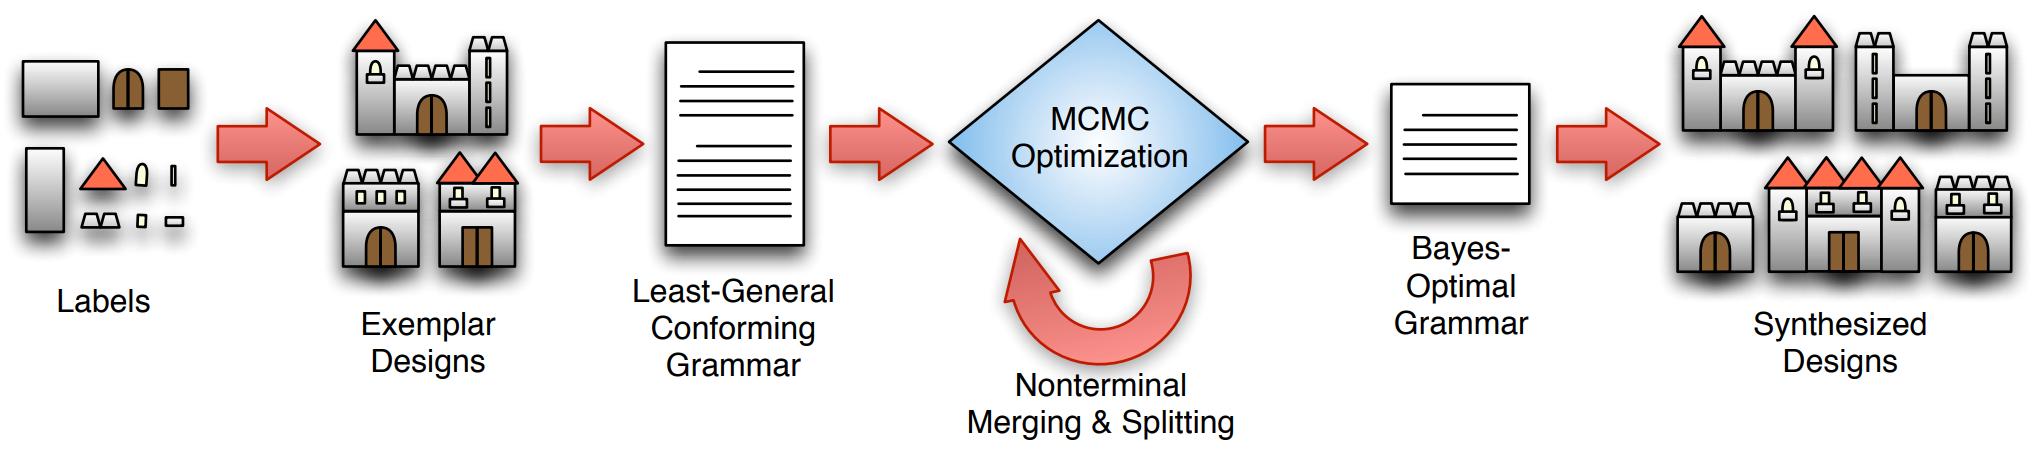
\includegraphics[width=12cm]{../images/talton_2012_system.PNG}
            \caption{Algorithmische Methode zum Lernen von Design Patterns}
        \end{figure}
    \end{frame}

    \begin{frame}
        \frametitle{Forschung: Verwandte Arbeiten}

        \begin{figure}
            \centering
            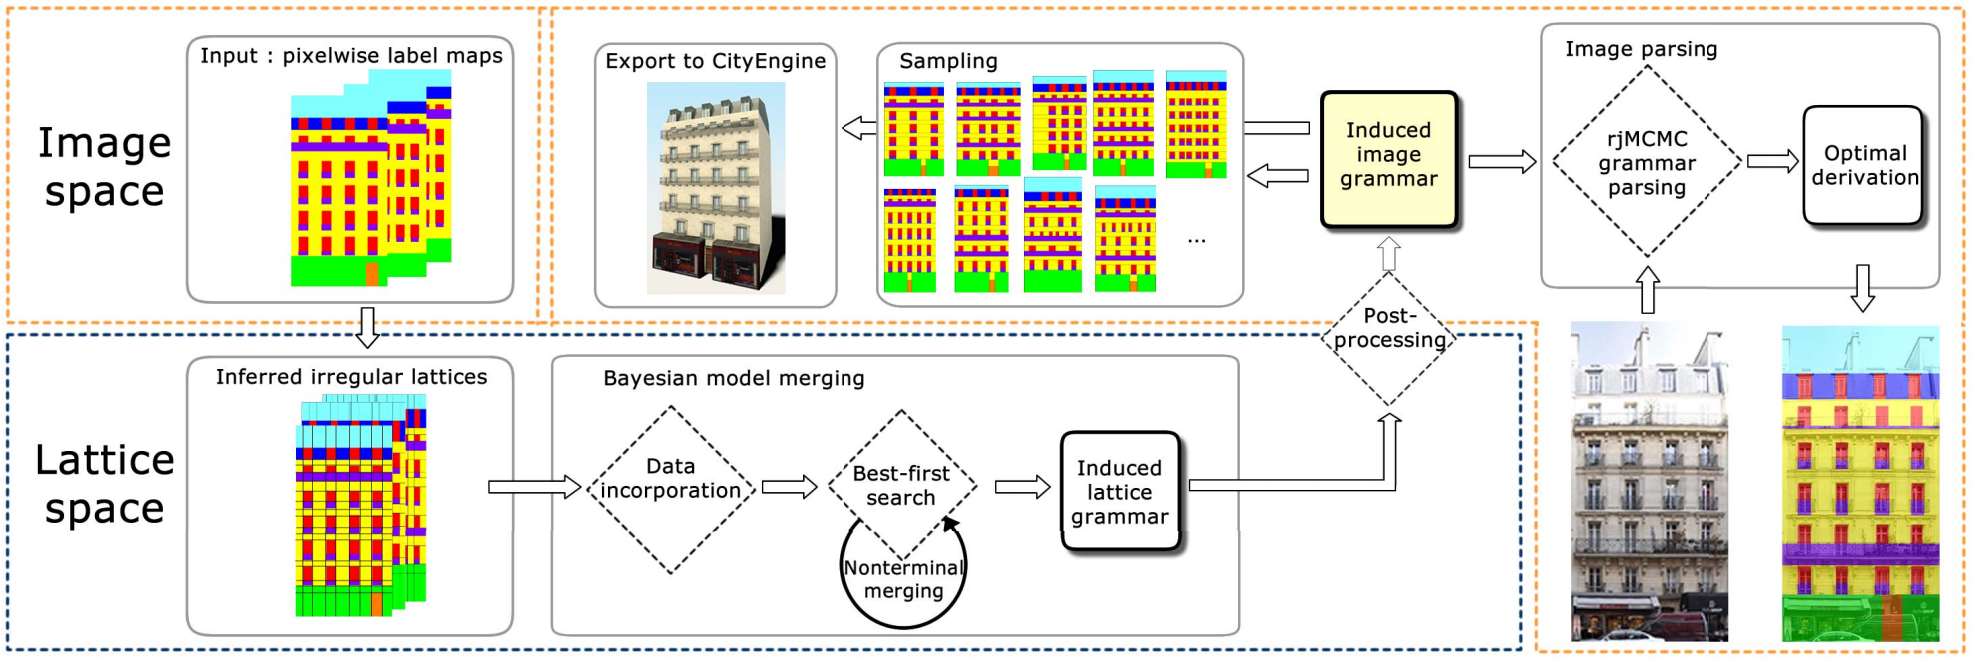
\includegraphics[width=12cm]{../images/martinovic_2013_system.PNG}
            \caption{Synthetisierung neuer Baustile und Rekonstruktion von Gebäuden}
        \end{figure}
    \end{frame}

    \begin{frame}
        \frametitle{Forschung: Verwandte Arbeiten}

        \begin{figure}
            \centering
            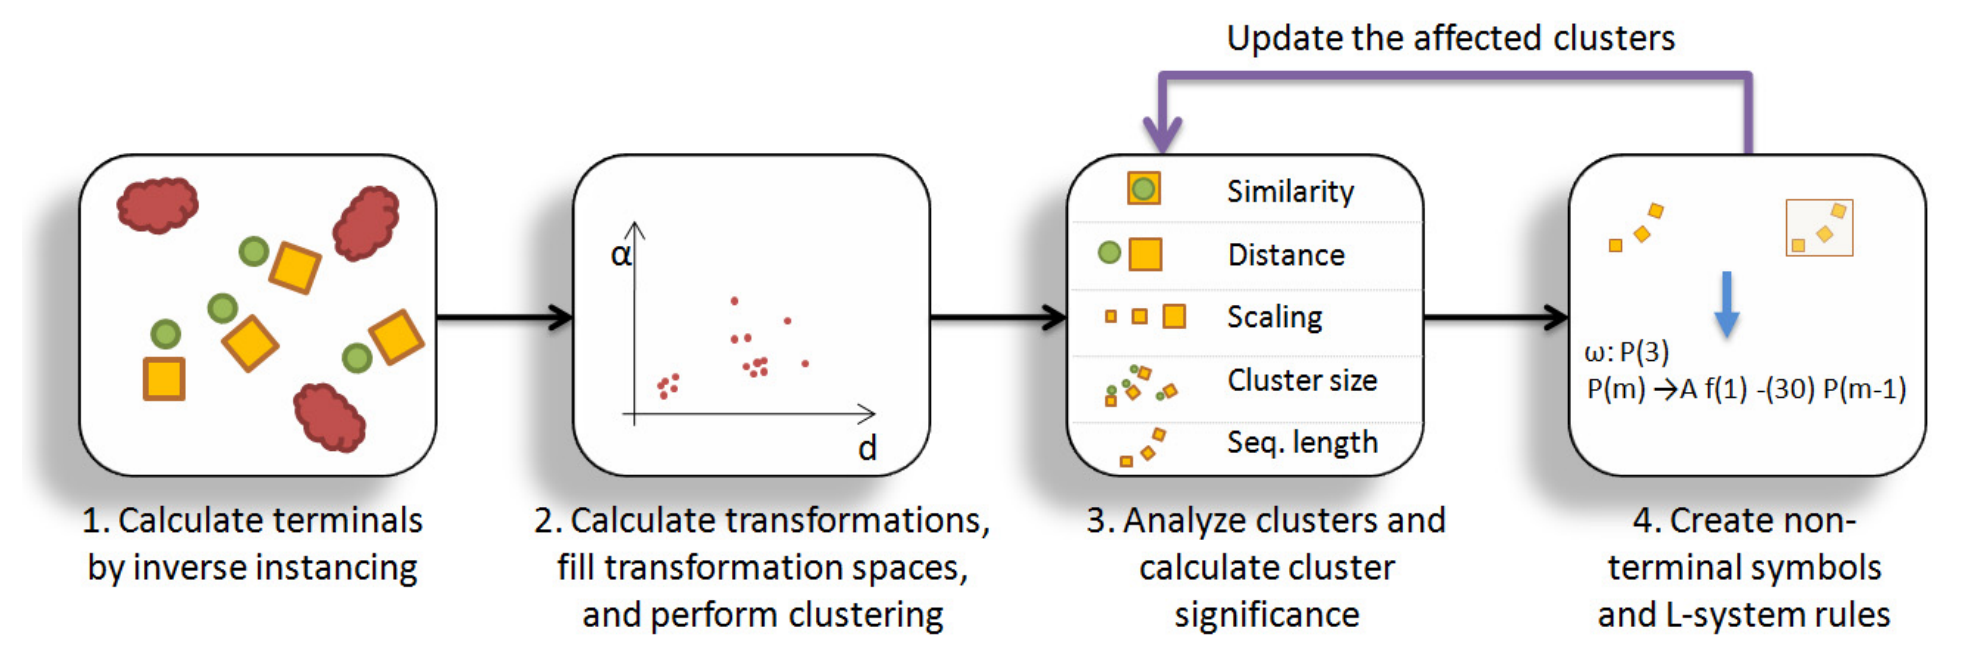
\includegraphics[width=12cm]{../images/stava_2010_system.PNG}
            \caption{System-Pipeline zur Erzeugung eines L-Systems eines 2D-Modells}
        \end{figure}
    \end{frame}

    \begin{frame}
        \frametitle{Forschung: Verwandte Arbeiten}

        \begin{figure}
            \centering
            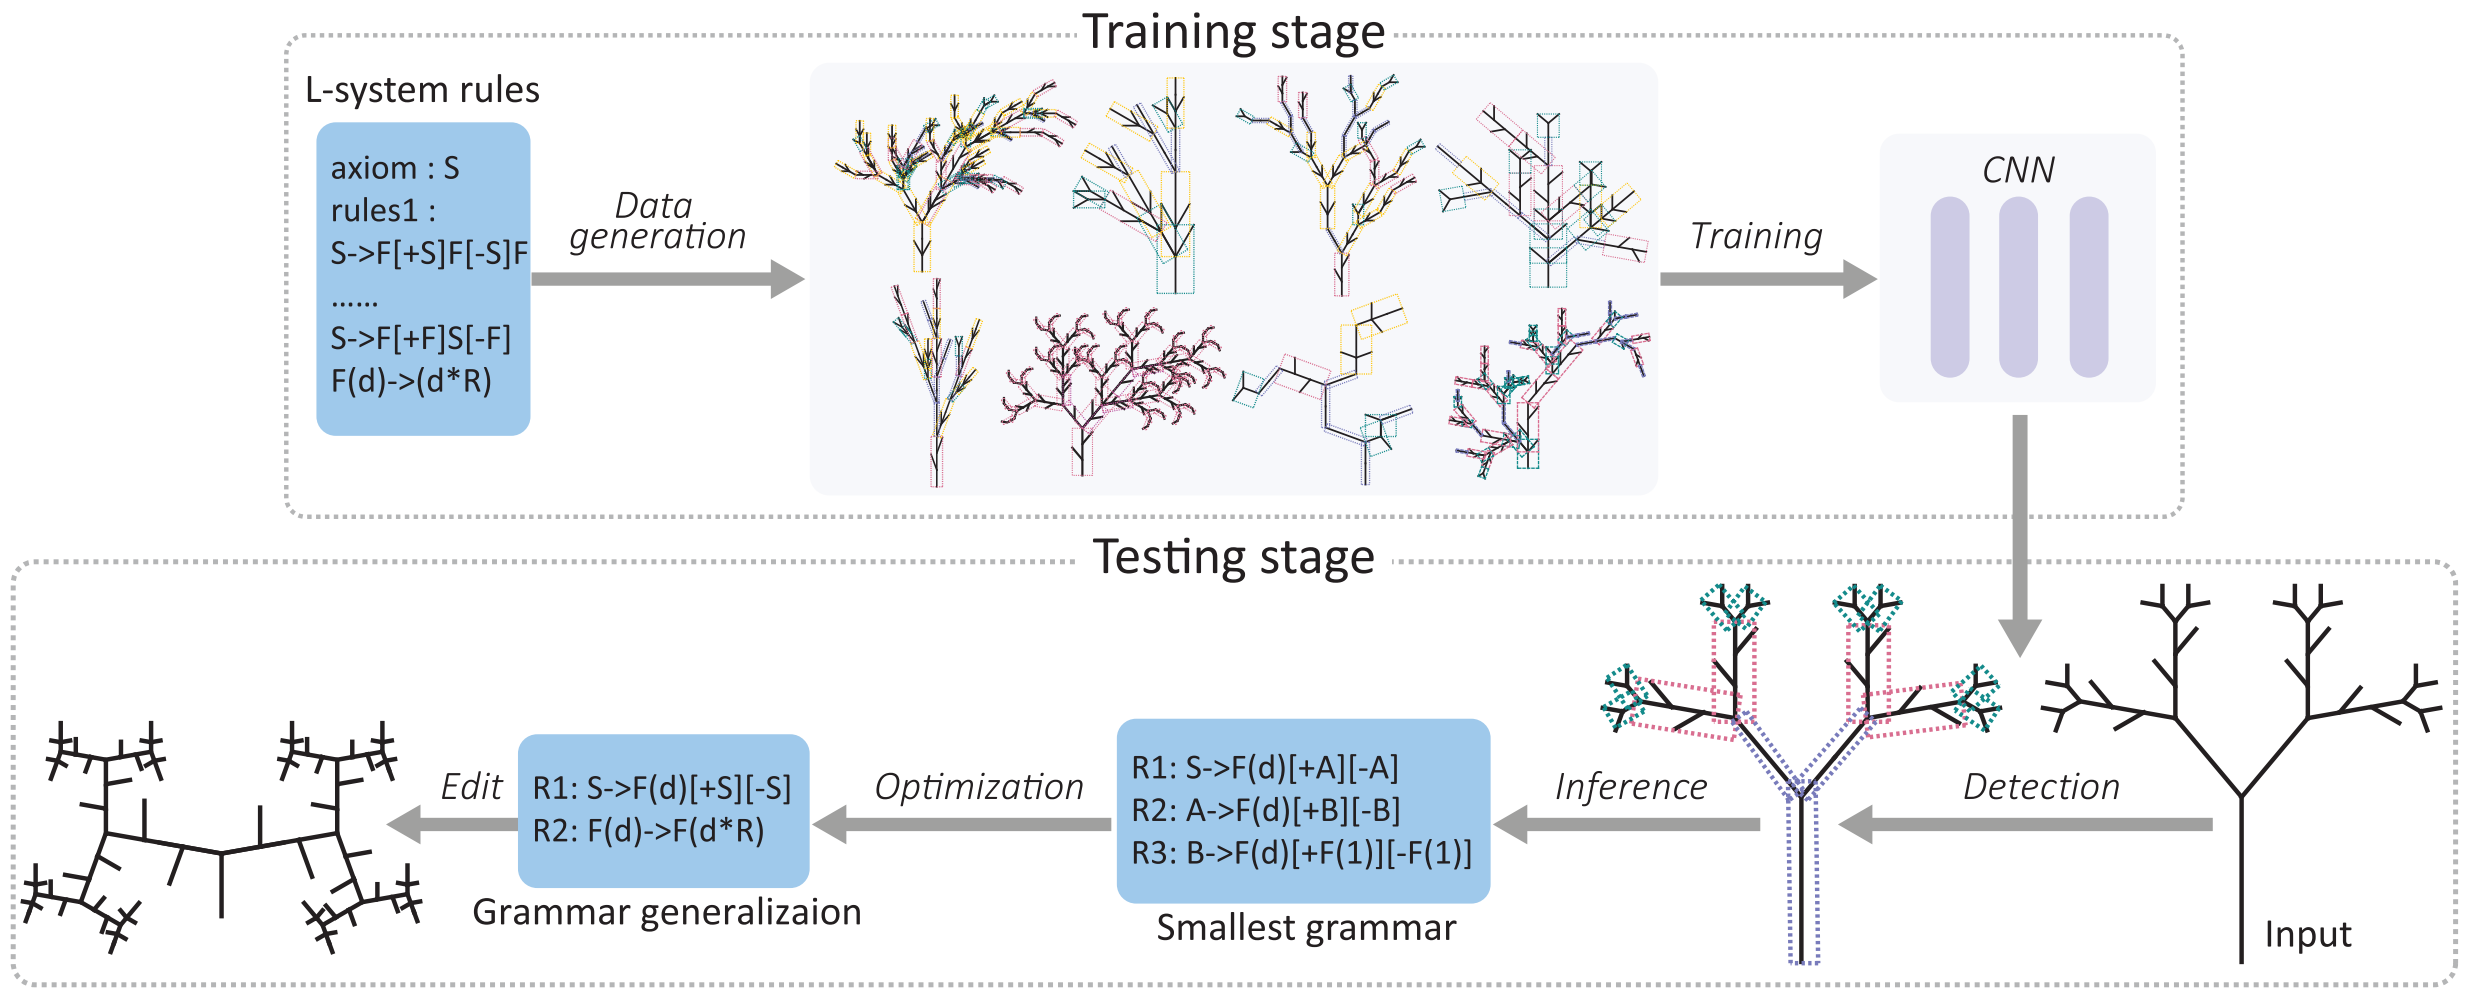
\includegraphics[width=12cm]{../images/guo_2020_system.PNG}
            \caption{Bearbeitung von L-System-Repräsentationen zur Erzeugung von Ähnlichkeit}
        \end{figure}
    \end{frame}

    \section{Methodik}
    \label{sec:methodik}
    \begin{frame}
        \frametitle{Methodik}

        \begin{figure}
            \centering
            
\includegraphics[width=10cm]{../images/methodik.jpg}
        \end{figure}
    \end{frame}

    \begin{frame}
        \frametitle{Methodik}

        \begin{itemize}
            \setlength\itemsep{1em}
            \item<1-> Strukturieren
            \item<2-> Datenaufbereitung
            \item<3-> Inferieren
        \end{itemize}
    \end{frame}

    \begin{frame}[allowframebreaks]
        \frametitle{Methodik: Inferieren}

        \underline{Initialisieren}\\
        ~\\
        \begin{algorithm}[H]
            $M=\{F,S\}$\\
            $\omega=S$\\
            $R \gets \{\alpha$: $S \rightarrow A\}$\\
            $\beta=$ nächster Knoten\\
            $M \gets \gamma \in \{A,B,\dots,Z\}$, mit $\gamma \notin M$\\
        \end{algorithm}

        \framebreak

        \begin{algorithm}[H]
            \While{true}{
                $\delta=$ Wort von $\beta$\\
                $\forall \{A,B,\dots,Z\} \setminus F \in \delta:$ Ersetze mit $\zeta \in \{A,B,\dots,Z\}$, mit $\zeta \notin M$\\
                $M \gets \zeta$\\
                $R \gets \{\gamma\rightarrow\delta\}$\\
                ~\\
                \eIf{$\exists\eta$ in $M\setminus\{F,S\}$ mit $\{\eta \rightarrow bel.\} \notin R$}{
                    $\gamma=\eta$
                }{
                    break
                }
                $\beta=$ nächster Knoten
            }
        \end{algorithm}
    \end{frame}

    \begin{frame}
        \frametitle{Methodik}

        \begin{itemize}
            \setlength\itemsep{1em}
            \item<1-> Strukturieren
            \item<1-> Datenaufbereitung
            \item<1-> Inferieren
            \item<2-> Komprimieren
        \end{itemize}
    \end{frame}

    \begin{frame}[allowframebreaks]
        \frametitle{Methodik: Komprimieren}

        \underline{Initialisieren}\\
        ~\\
        \begin{algorithm}[H]
            $\mathcal{L}^+ \leftarrow L_s$\\
            $\mathcal{L}=\emptyset$\\
            $w_l \in [0,1]$\\
            Finde maximalen Unterbaum $T'$ aus $T$ mit Wiederholungen $n>1$
        \end{algorithm}

        \framebreak

        \begin{algorithm}[H]
            \While{true}{
                Ersetze alle Vorkommen von $T'$ mit demselben Symbol $\gamma \in \{A,B,\dots,Z\}$\\
                $R \leftarrow \{\gamma \rightarrow L_s\}$ mit $L_s$ aus $T'$, $R$ aus $\mathcal{L}$\\
                \If{$C_i(\mathcal{L}) \geq C_i(\mathcal{L}^+)$}{
                    break
                }
                $T \leftarrow T'$\\
                $\mathcal{L}^+ \leftarrow \mathcal{L}$\\
                Finde maximalen Unterbaum $T'$ aus $T$ mit Wiederholungen $n>1$
            }
        \end{algorithm}

        \framebreak

        \begin{algorithm}[H]
            \centering
            $C_i(\mathcal{L})= \sum\limits_{A(P) \rightarrow M^* \in \mathcal{L}} w_l * |M^*| + (1 - w_l) * N(A(P)\rightarrow M^*)$
        \end{algorithm}
    \end{frame}

    \begin{frame}
        \frametitle{Methodik}

        \begin{itemize}
            \setlength\itemsep{1em}
            \item<1-> Strukturieren
            \item<1-> Datenaufbereitung
            \item<1-> Inferieren
            \item<1-> Komprimieren
            \item<2-> Generalisieren
        \end{itemize}
    \end{frame}

    \begin{frame}[allowframebreaks]
        \frametitle{Methodik: Generalisieren}

        \underline{Initialisieren}\\
        ~\\
        \begin{algorithm}[H]
            Regelpaar $p^* = \emptyset$\\
            $\mathcal{L}^* = \mathcal{L}^+$\\
            $C_g^{old} = C_g(\mathcal{L}^* + \{p^*\}, \mathcal{L}^*)$
        \end{algorithm}

        \framebreak

        \begin{algorithm}[H]
            \While{true}{
                Finde Regelpaar $p^*$ mit minimalen Kosten $C_g(\mathcal{L}^* + \{p_i\}, \mathcal{L}^*),$\\
                ~~~~$\forall p_i \in \mathcal{P}$\\
                \If{$C_g(\mathcal{L}^* + \{p^*\}, \mathcal{L}^*) \geq 0$}
                {
                    break
                }
                $c^* = C_g(\mathcal{L}^* + \{p^*\}, \mathcal{L}^*) - C_g^{old}$\\
                $C_g^{old} = C_g(\mathcal{L}^* + \{p^*\}, \mathcal{L}^*)$\\
                $\mathcal{L}^* = \mathcal{L}^* + \{p^*\}$\\
                \If{$c^* > 0$}
                {
                    break
                }
            }
        \end{algorithm}

        \framebreak

        \begin{algorithm}[H]
            $L(\mathcal{L}) = |M| + \sum\limits_{A(P) \rightarrow M^* \in \mathcal{L}} |M^*|$
            \\~\\
            \\~\\
            $D_g(\mathcal{L}^+, \mathcal{L}^*)= \sum\limits_{(A(P) \rightarrow M^*_A , B(P) \rightarrow M^*_B) \in M(\mathcal{L^+} \rightarrow \mathcal{L^*})} D_s(M^*_A, M^*_B)$\\
            \\~\\
            \\~\\
            $C_g(\mathcal{L}^*, \mathcal{L}^+) = w_0 * (L(\mathcal{L}^*) - L(\mathcal{L}^+)) + (1 - w_0) + D_g(\mathcal{L}^+, \mathcal{L}^*)$
        \end{algorithm}
    \end{frame}

    \begin{frame}
        \frametitle{Methodik}

        \begin{columns}
            \column{0.5\textwidth}
            \begin{itemize}
                \setlength\itemsep{1em}
                \item<1-> Strukturieren
                \item<1-> Datenaufbereitung
                \item<1-> Inferieren
                \item<1-> Komprimieren
                \item<1-> Generalisieren
            \end{itemize}
            \column{0.5\textwidth}
            \begin{itemize}
                \setlength\itemsep{1em}
                \item<2-> Visualisieren
                \item<3-> Randomisieren
            \end{itemize}
        \end{columns}
    \end{frame}

    \section{Ergebnisse}
    \label{sec:ergebnisse}
    \begin{frame}
        \frametitle{Ergebnisse}

        \begin{figure}
            \centering
            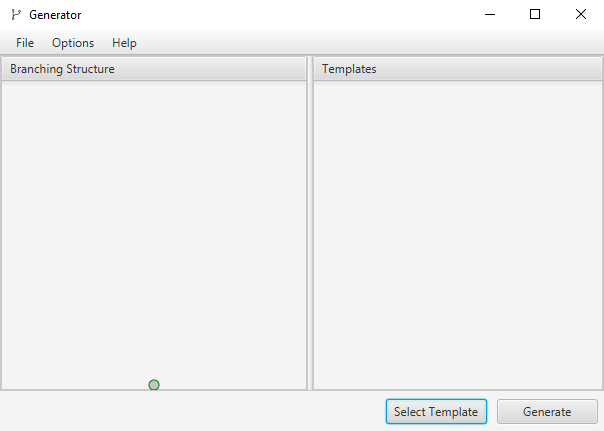
\includegraphics[width=8cm,cfbox=blue 0.4pt 1pt]{../images/UI.PNG}
            \caption{Umgesetztes Programm}
        \end{figure}
    \end{frame}

    \section{Fazit}
    \label{sec:fazit}
    \begin{frame}
        \frametitle{Fazit}

        \begin{figure}
            \centering
            
\includegraphics[width=10cm]{../images/fazit.jpg}
        \end{figure}
    \end{frame}

    \begin{frame}
        \frametitle{Fazit}

        \begin{itemize}
            \setlength\itemsep{1em}
            \item Algorithmen liefern zufriedenstellende Ergebnisse (subjektiv)
            \item
        \end{itemize}
    \end{frame}

\end{document}